\section{Συστήματα Κοινής και Κατανεμημένης Μνήμης}
\paragraph{}
Με βάση την οργάνωση της μνήμης τους, τα πολυπύρηνα συστήματα χωρίζονται σε κοινής μνήμης (shared memory) και κατανεμημένης μνήμης (distributed memory). Στις αρχιτεκτονικές κοινής μνήμης οι επεξεργαστές του συστήματος προσπελαύνουν όλοι την ίδια φυσική μνήμη και τις περισσότερες φορές η διασύνδεσης τους γίνεται μέσω ενός διαδρόμου (memory bus) βλ. Σχήμα \ref{fig:SMP}. Αντίθετα, στις αρχιτεκτονικές κατανεμημένης μνήμης κάθε επεξεργαστής έχει τη δική του ιδιωτική μνήμη, και η επικοινωνία μεταξύ τους γίνεται πάνω από κάποιο δίκτυο διασύνδεσης βλ. Σχήμα  \ref{fig:cluster}.

\begin{figure}
    \centering
    \begin{subfigure}[b]{0.45\textwidth}
        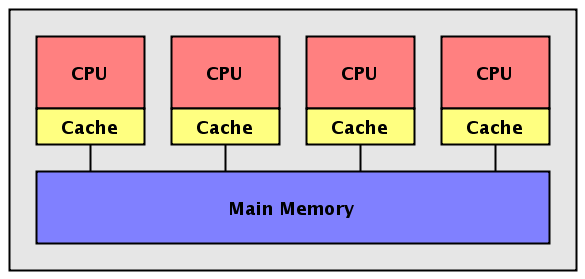
\includegraphics[width=\textwidth]{./images/SMP.png}
        \caption{Κοινής Μνήμης}
        \label{fig:SMP}
    \end{subfigure}
    \quad %add desired spacing between images, e. g. ~, \quad, \qquad, \hfill etc. 
      %(or a blank line to force the subfigure onto a new line)
    \begin{subfigure}[b]{0.45\textwidth}
        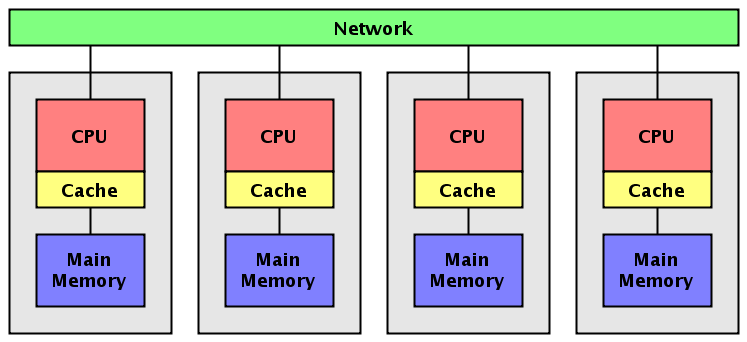
\includegraphics[width=\textwidth]{./images/cluster.png}
        \caption{Κατανεμημένης Μνήμης}
        \label{fig:cluster}
    \end{subfigure}
    \caption{Αναπαράσταση συστημάτων κοινής και κατανεμημένης μνήμης}
\end{figure}
\paragraph{}
Ανάλογα με την οργάνωση τους, οι αρχιτεκτονικές κοινής μνήμης χωρίζονται σε δύο κατηγορίες. Η πρώτη κατηγορία αφορά περιπτώσεις όπου ο χρόνος πρόσβασης στη μνήμη είναι σταθερός και ονομάζεται Ομοιόμορφης Πρόσβασης στη Μνήμη(Uniform Memory Access-UMA). Σε αυτή την περίπτωση ο επεξεργαστής, και το block που προσπελαύνει, δεν επηρεάζουν το χρόνο πρόσβασης στη μνήμη. Στη δεύτερη κατηγορία εμπίπτουν τα συστήματα όπου η κοινή μνήμη είναι κατανεμημένη στους επεξεργαστές και επιπλέον υλικό φροντίζει για την πρόσβαση των επεξεργαστών σε μη τοπικές μνήμες. Είναι προφανές ότι πλέον ο χρόνος πρόσβασης δεν είναι σταθερός. Έτσι τα συστήματα αυτά ονομάζονται Μη-Ομοιόμορφης Πρόσβασης στη Μνήμη(Non-Uniform Memory Access-NUMA). Μία οπτική αναπαράσταση για τις δύο κατηγορίες δίνεται στο Σχήμα \ref{fig:shared_mem}.\footnote{Εικόνες από: www.sqlskills.com/blogs/jonathan/understanding-non-uniform-memory-accessarchitectures-numa}

\begin{figure}
    \centering
    \begin{subfigure}[b]{0.45\textwidth}
        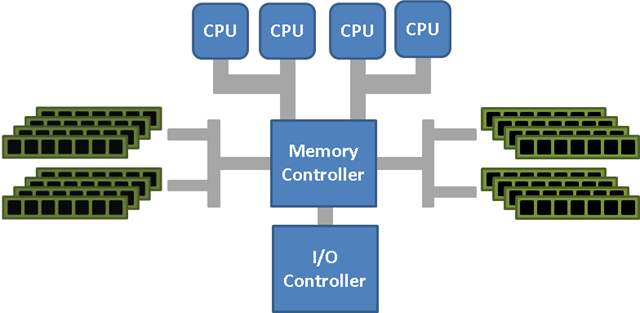
\includegraphics[width=\textwidth]{./images/UMA.png}
        \caption{UMA}
    \end{subfigure}
    \quad %add desired spacing between images, e. g. ~, \quad, \qquad, \hfill etc. 
      %(or a blank line to force the subfigure onto a new line)
    \begin{subfigure}[b]{0.45\textwidth}
        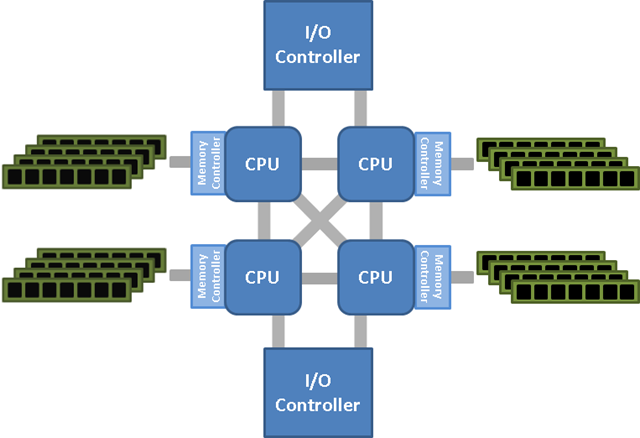
\includegraphics[width=\textwidth]{./images/NUMA.png}
        \caption{NUMA}
    \end{subfigure}
    \caption{Κατηγορίες Αρχιτεκτονικών Κοινής Μνήμης}
    \label{fig:shared_mem}
\end{figure}

\paragraph{}
Οι σύγχρονοι υπερυπολογιστές χρησιμοποιούν συνδυασμούς των δύο παραπάνω δημιουργώντας υβριδικές αρχιτεκτονικές. Συνήθως οι κόμβοι\footnote{Με τον όρο κόμβοι θα αναφερόμαστε στο κομμάτι του συστήματος που είναι συνδεδεμένο στο δίκτυο διασύνδεσης} τους αποτελούνται από εμπορικούς επεξεργαστές, επιταχυντές γραφικών ή co-processors όπως ο Xeon Phi. Καθώς προσεγγίζουμε την εποχή του exascale computing, στην οποία ένας υπερυπολογιστής θα έχει την δυνατότητα να εκτελέσει ένα τρισεκατομμύριο πράξεις κινητής υποδιαστολής το δευτερόλεπτο, οι σχεδιαστές των μηχανημάτων έχουν την τάση να σχεδιάζουν συστήματα στα οποία  κάθε κόμβος έχει πάρα πολλούς <<αδύναμους>> πυρήνες και ακόμα περισσότερα νήματα. Τέσσερις από τους δέκα ισχυρότερους υπολογιστές του κόσμου για το 2015, συνδυάζουν σε κάθε κόμβο ένα απλό επεξεργαστή με αρχιτεκτονική κοινού χώρου διευθύνσεων με ένα co-processor που περιέχει δεκάδες επεξεργαστές. Αυτά τα δύο είναι συνδεδεμένα μεταξύ τους, συνήθως μέσω PCIe, σχηματίζοντας ένα κόμβο που συνδέεται με άλλους μέσω κάποιου εξελιγμένου δικτύου διασύνδεσης 

\paragraph{}
Δύο παραδείγματα υπερυπολογιστών, σε φάση κατασκευής, που υλοποιούν την πιο πάνω υβριδική αρχιτεκτονική είναι ο Theta από το Argonne National Laboratory και ο Cori από το National Energy Research Scientific Computing Center. Και οι δύο χρησιμοποιούν ένα συνδυασμό Intel Xeon με Intel Xeon Phi σε κάθε κόμβο, που τελικά περιέχει πάνω από 70 πυρήνες ή 280 νήματα. Επιπλέον, η τάση αυτή φαίνεται να ενισχύεται, με ιθύνοντες της Intel να υποστηρίζουν ότι ο πρώτος exascale υπολογιστής θα περιέχει χιλιάδες πυρήνες σε κάθε κόμβο\footnote{http://www.nextplatform.com/2015/08/12/future-systems-intel-fellow-conjures-the-perfect-exascale-machine/} με το UC Davis να έχει ήδη αναπτύξει τον πρώτο επεξεργαστή με χίλιους πυρήνες.\footnote{https://www.ucdavis.edu/news/worlds-first-1000-processor-chip}

\paragraph{}
Ωστόσο, το συνονθύλευμα αυτών των αρχιτεκτονικών οδηγεί σε μία περίπλοκη ιεραρχία μνήμης. Κάθε πυρήνας έχει κάποια ιδιωτική  κρυφή μνήμη (cache) για μερικά επίπεδα. Σε επόμενο στάδιο, ανάλογα με τον πυρήνα, μπορεί να υπάρχει κοινό επίπεδο cache για όλους τους πυρήνες που βρίσκονται στον ίδιο επεξεργαστή ή κάποια άλλου είδους επικοινωνία για πυρήνες στο ίδιο package. Στην περίπτωση του Xeon Phi, ένας δακτύλιος δύο κατευθύνσεων συνδέει τους πυρήνες μεταξύ τους και με μνήμη on the package (DDR5 ή custom made). Σε επόμενα επίπεδα συναντάμε την κύρια μνήμη, μνήμες όπως NVRAM και μαγνητικούς σκληρούς δίσκους για μόνιμη αποθήκευση, ενώ στο τελευταίο επίπεδο συνήθως βρίσκουμε μαγνητικές ταινίες που αποσκοπούν σε μακροπρόθεσμη αποθήκευση κυρίως για σκοπούς αντιγράφων ασφαλείας. 

\paragraph{}
Αυτή η βαθιά ιεραρχία μνήμης εισάγει νέες προκλήσεις. Πλέον η θέση της διεργασίας στο μηχάνημα θα είναι όλο και πιο κρίσιμη για την επικοινωνία της. Ανάλογα με τη θέση της διεργασίας που καλείται να ανταλλάξει δεδομένα, διαφορετικά πρότυπα επικοινωνίας θα λαμβάνουν χώρα.

\paragraph{}
Μία από τις προσπάθειες για αντιμετώπιση των προκλήσεων που εμφανίζονται καθώς οδεύουμε στην εποχή του exascale, είναι το Ευρωπαϊκό ερευνητικό πρότζεκτ Exanode. Πρόκειται για την προσπάθεια της επιστημονικής κοινότητας να σχεδιάσει τον ιδανικό κόμβο. Θα είναι βασισμένος στην αρχιτεκτονική του ARM-v8 ενώ θα περιέχει μνήμη που θα υποστηρίζει κλιμακωσιμότητα για τον exascale υπολογιστή. 

\section{Παράλληλα Προγραμματιστικά Μοντέλα}
\paragraph{}
Για κάθε αρχιτεκτονική που αναφερθήκαμε έχουν αναπτυχθεί και ανάλογα προγραμματιστικά μοντέλα. Έτσι έχουμε το μοντέλο κοινού χώρου διευθύνσεων, το μοντέλο ανταλλαγής μηνυμάτων για συστήματα κατανεμημένης μνήμης και το υβριδικό μοντέλο που συνδυάζει τα δύο προηγούμενα. Στόχος τους είναι να παρέχουν στους προγραμματιστές ευκολία στη γραφή κώδικα, χωρίς να τους επιβαρύνουν με λεπτομέρειες της υλοποίησης αλλά ταυτόχρονα να εκμεταλλεύονται όσο το δυνατό περισσότερο τα πλεονεκτήματα και τα χαρακτηριστικά της κάθε αρχιτεκτονικής.
\subsection{Μοντέλο κοινού χώρου διευθύνσεων}
\paragraph{}
Το μοντέλο αυτό είναι σχεδιασμένο για αρχιτεκτονικές κοινού χώρου διευθύνσεων. Καθώς όλες οι διεργασίες έχουν πρόσβαση στην ίδια μνήμη, η επικοινωνία μεταξύ τους γίνεται ασύγχρονα μέσω πρόσβασης σε κοινές θέσης μνήμης. Ωστόσο, ταυτόχρονες προσβάσεις στην ίδια θέση μνήμης ενδέχεται να δημιουργήσουν καταστάσεις ανταγωνισμού (race conditions), με τη χρήση σχημάτων συγχρονισμού να είναι απαραίτητη. Πρόκειται αδιαμφισβήτητα για το πιο απλό μοντέλο από προγραμματιστική σκοπιά, με τις εκάστοτε υλοποιήσεις να αναλαμβάνουν να επιλύσουν θέματα συγχρονισμού. Υπάρχουν ποικίλες υλοποιήσεις του μοντέλου (OpenMP, Cilk, Thread Building Blocks) με την πιο ευρέως διαδεδομένη την OpenMP.

\subsection{Μοντέλο Ανταλλαγής Μηνυμάτων}
\paragraph{}
Το μοντέλο αυτό αποσκοπεί στην υλοποίηση της επικοινωνίας μεταξύ διεργασιών όπου η μνήμη του συστήματος είναι κατανεμημένη. Οι διεργασίες επικοινωνούν μεταξύ τους ανταλλάσσοντας μηνύματα μέσω ποικίλων εντολών. Η κλήση των εντολών γίνεται από τον προγραμματιστή, δίνοντας του έτσι την ευχέρεια να ορίσει ποιες διεργασίες θα επικοινωνήσουν, τα δεδομένα που θα ανταλλάξουν και σε ποιο στάδιο της εκτέλεσης να θα γίνει επικοινωνία. Στην πιο απλή μορφή της, μια εντολή με σκοπό την αποστολή δεδομένων περιλαμβάνει τη διεύθυνση ενός τοπικού buffer με τα δεδομένα, το αναγνωριστικό της διεργασίας-παραλήπτη και τον τύπο των δεδομένων που αποστέλνονται. Αναλογικά, μία εντολή λήψης δεδομένων, περιλαμβάνει ένα buffer για την αποθήκευση των εισερχόμενων δεδομένων, το αναγνωριστικό της διεργασίας-αποστολέα και τον τύπο των δεδομένων που παραλαμβάνονται.


\paragraph{}
Επιπλέον, το μοντέλο ανταλλαγής μηνυμάτων υποστηρίζει διάφορα είδη επικοινωνίας. Ένα είδος είναι η σύγχρονη (blocking) όπου οι διεργασίες συγχρονίζονται κατά την αποστολή των δεδομένων. Ουσιαστικά, με την κλήση των συναρτήσεων send, από τη διεργασία-αποστολέα, και receive, από τη διεργασία-παραλήπτη,  οι διεργασίες αναστέλλουν τη λειτουργία τους εώς το πέρας της επικοινωνίας. Αντίθετα, στην ασύγχρονη επικοινωνία (non-blocking) οι κλήσεις send και receive επιστρέφουν όσο το δυνατό γρηγορότερα, έχοντας αναθέσει την αποστολή και λήψη των δεδομένων σε κάποιο άλλο μηχανισμό, χωρίς η επικοινωνία να έχει ολοκληρωθεί. Σε επόμενο στάδιο, κάποια συνάρτηση τύπου wait καλείται πριν κάποια από τις διεργασίες προσπελάσει τα νέα δεδομένα για να διασφαλιστεί ότι έχουν ληφθεί. Αν το υλικό το επιτρέπει και οι μηχανισμοί που αναλαμβάνουν την αποπεράτωση της διαδικασίας είναι ανεξάρτητοι από την εκτέλεση της διεργασίας, η non-blocking επικοινωνία επιτρέπει σε υπολογισμούς και επικοινωνία να γίνουν ταυτόχρονα. 

\paragraph{}
Μία άλλη διάκριση μεταξύ των ειδών επικοινωνίας είναι η σημείο-προς-σημείο (point-to-point) και η συλλογική επικοινωνία (collectives). Στην επικοινωνία point-to-point συμμετέχουν μόνο δύο διεργασίες, μία που αποστέλλει και μία που λαμβάνει δεδομένα. Στα collectives μπορούν να λαμβάνουν μέρος περισσότερες από δύο διεργασίες. Τέτοιου είδους επικοινωνία είναι συνηθισμένη όταν μια διεργασία καλείται να αποστείλει δεδομένα σε πολλές διεργασίες ή αντίθετα, να λάβει δεδομένα από διάφορες διεργασίες.

\paragraph{}
Υπάρχουν επίσης, πολλές υλοποιήσεις αυτού του προγραμματιστικού μοντέλου, με τις περισσότερες να ακολουθούν το πρότυπο MPI(Message Passing Interface) που αναπτύσσεται από το MPI forum \cite{MPI}. Το πρότυπο αυτό καθορίζει τις λειτουργίες που πρέπει να προσφέρει μία υλοποίηση του μοντέλου. Διασημότερες υλοποιήσεις είναι το OpenMPI \cite{OMPI} και το MPICH \cite{MPICH}. Στα πειράματα μας επιλέξαμε να χρησιμοποιήσουμε το OpenMPI, καθώς ενσωματώνει νέα χαρακτηριστικά πολύ γρήγορα και παραμένει σε μεγάλο βαθμό ερευνητικό εργαλείο.
\subsection{Υβριδικό Μοντέλο}
Στις περισσότερες εφαρμογές που προορίζονται για εκτέλεση σε υπερυπολογιστές, χρησιμοποιείται το υβριδικό μοντέλο, που συνδυάζει MPI με κάποια υλοποίηση του μοντέλου κοινού χώρου διευθύνσεων. Για επικοινωνία μεταξύ των διεργασιών που βρίσκονται στον ίδιο κόμβο(intranode communication), χρησιμοποιείται κάποια υλοποίηση του μοντέλου κοινού χώρου διευθύνσεων με σκοπό την αποφυγή επιπλέον χρόνου επικοινωνίας,  που εισάγουν οι πιο περίπλοκες υλοποιήσεις του MPI (communication overhead). Για επικοινωνία των διεργασιών που βρίσκονται σε διαφορετικούς κόμβους(internode communication) χρησιμοποιείται το MPI. Ωστόσο η χρήση δύο μοντέλων επικοινωνίας δυσχεραίνει το έργο των προγραμματιστών, ενώ οι υλοποιήσεις χρειάζονται πολύ tuning για να πετύχουν καλή επίδοση.


\section{Χρήση MPI για επικοινωνία σε κοινό χώρο διευθύνσεων}

\paragraph{}
Καθώς νέες εκδόσεις του MPI αναπτύσσονται, το overhead από τη χρήση του μειώνεται, κάνοντας πιο ελκυστική τη χρήση του και για την επικοινωνία διεργασιών μέσα στον κόμβο. Έτσι δίνεται στους προγραμματιστές η δυνατότητα να κάνουν χρήση μόνο του MPI για όλη την επικοινωνία της εφαρμογής. Επιπρόσθετα, έχουν περισσότερο έλεγχο στην κατανομή των διεργασιών στους υπολογιστικούς πόρους, ενώ εφαρμογές αναπτυγμένες στο μοντέλο MPI, δεν χρειάζονται μεταβολή σε υβριδικό προγραμματιστικό μοντέλο για να εκτελεστούν αποδοτικά σε υπερυπολογιστές. 

\paragraph{}
Πολλές ερευνητικές προσπάθειες επικεντρώνονται στη βελτιστοποίηση της intranode επικοινωνίας του MPI. Στις τελευταίες εκδόσεις του, έγιναν προσθήκες οι οποίες επιτρέπουν στις intranode διεργασίες να επικοινωνούν με χαμηλή καθυστέρηση, κάνοντας χρήση της κοινής τους μνήμης. Ωστόσο αυτές οι υλοποιήσεις περιλαμβάνουν την δέσμευση buffers από το MPI, αντιγραφή των δεδομένων εκεί και μετέπειτα αντιγραφή στον τελικό buffer. Για μεγάλα μηνύματα η διαδικασία αυτή οδηγεί σε έξωση δυνητικά χρήσιμων δεδομένων από την cache, χωρίς να είναι απαραίτητο.

 \paragraph{}
Με σκοπό να βελτιώσουν το χρόνο επικοινωνίας intranode διεργασιών για μεγάλα μήνυματα, οι B. Goglin και S. Moreaud ανάπτυξαν το Kernel Nemesis (KNEM) \cite{KNEM}. Πρόκειται για ένα δομοστοιχείο (module) σχεδιασμένο για τον πυρήνα του λειτουργικού συστήματος Linux που παρέχει στις υλοποιήσεις MPI την δυνατότητα να εκτελούν μεταφορά δεδομένων ανάμεσα σε τοπικές διεργασίες μέσω μόνο μίας αντιγραφής(single-copy data transfer). Αφού δεν απαιτεί τη δέσμευση ενδιαμέσων buffers όπως οι naive υλοποιήσεις του MPI μειώνεται σημαντικά το overhead της intranode επικοινωνίας. Είναι ανεξάρτητο του υλικού, ενώ υποστηρίζει point-to-point και collective επικοινωνία. 
\begin{figure}[h]
    \centering
    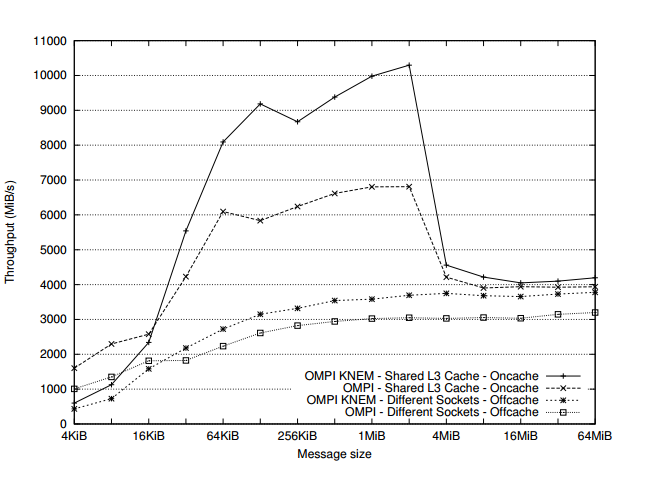
\includegraphics[width=\textwidth]{./images/knem_graph.png}
    \caption{Thoughtput για το IMB PingPong Benchmark}
    \label{fig:Knem}
\end{figure}
\paragraph{}
Στο Σχήμα \ref{fig:Knem} φαίνεται η αύξηση στο ρυθμό ανταλλαγής δεδομένων με χρήση του KNEM για το benchmark IMB PingPong σε ένα NUMA μηχάνημα. Οι περιπτώσεις με όνομα \textit{Shared Cache - Oncache} αφορούν την πιο φιλική προς την cache προσέγγιση, στις οποίες οι διεργασίες που επικοινωνούν μοιράζονται μία μεγάλη cache. Αντίθετα οι περιπτώσεις \textit{Different Sockets - Offcache}, αντιστοιχούν στο χειρότερο σενάριο όπου δεν υπάρχει κοινή cache μεταξύ των διεργασιών.
\paragraph{}
Από το σχήμα φαίνεται ότι στις περιπτώσεις που δεν υπάρχει κοινή cache η επίδοση της επικοινωνίας βελτιώνεται με χρήση του KNEM, καθώς η απώλεια κοινής cache έχει ελάχιστη επίδραση στη Single-Copy διαδικασία που εκτελεί, αντίθετα με την Double-Copy και τους ενδιάμεσους buffers. Όσον αφορά τις περιπτώσεις που υπάρχει κοινή cache, το KNEM υστερεί των υπαρχόντων υλοποιήσεων για μηνύματα με μέγεθος μικρότερα της χωρητικότητας της cache. Κάτι τέτοιο είναι αναμενόμενο καθώς το KNEM εκτελεί κλήσεις συστήματος που εισάγουν σημαντικό overhead στη διαδικασία. Ωστόσο, για μηνύματα με μέγεθος μεγαλύτερο από τη χωρητικότητα της cache το KNEM υπερέχει σημαντικά. Η συνήθης πρακτική είναι η χρήση του KNEM για μεγέθη μηνυμάτων μεγαλύτερα από 4ΚΒ.

\paragraph{}
Εκτός από τη βελτιστοποίηση της point-to-point επικοινωνίας, η επιστημονική κοινότητα ασχολήθηκε και με την collective. Συγκεκριμένα ο S. Li και άλλοι \cite{Sli}, πρότειναν αλγόριθμους για την υλοποίηση συγκεκριμένων collectives (allreduce, reduce, broadcast) σχεδιασμένους ειδικά για αρχιτεκτονική NUMA. Με τη χρήση των αλγορίθμων επιτυγχάνουν κατά μέσο όρο 2.5 φορές καλύτερη επίδοση σε σχέση με τους γενικούς αλγορίθμους που χρησιμοποιούν οι υλοποιήσεις του MPI. Επιπλέον, γίνεται και σύγκριση της επίδοσης με OpenMP με τα αποτελέσματα να υπερέχουν με τη χρήση του MPI και των προσαρμοσμένων αλγορίθμων. 

\section{Κίνητρο}
\paragraph{}
Όπως αναφέραμε πιο πάνω, η εμφάνιση multicore και manycore επεξεργαστών αύξησε το επίπεδο του παραλληλισμού εσωτερικά των κόμβων. Καθώς ο αριθμός των πυρήνων μέσα στους κόμβους συνεχίζει να αυξάνει, η intranode επικοινωνία θα έχει μεγαλύτερο αντίκτυπο στον τελικό χρόνο εκτέλεσης. Συνεπώς, η πρόβλεψη του χρόνου επικοινωνίας σε αρχιτεκτονικές κοινής μνήμης αποκτά όλο και περισσότερη χρησιμότητα.
\begin{figure}[t]
    \centering
    \captionsetup{justification=centering,margin=0cm}
    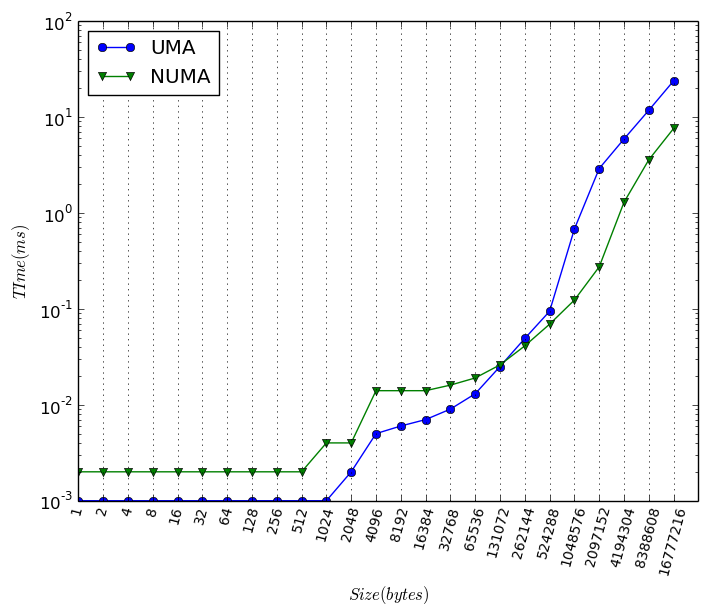
\includegraphics[width=\textwidth]{./images/NUMAvsUMA.png}
    \caption{Συγκριτικό διάγραμμα για τις αρχιτεκτονικές UMA και NUMA για point-to-point επικοινωνία}
    \label{fig:UMAvsNUMA}
\end{figure}
\paragraph{}
Στο Σχημα \ref{fig:UMAvsNUMA} φαίνεται ο χρόνος επικοινωνίας που αναλώνεται για επικοινωνία για ένα απλό benchmark σε αρχιτεκτονικές UMA και NUMA για 8 διεργασίες. Στο benchmark γίνεται ping-pong point-to-point επικοινωνία ανά δύο διεργασίες. Για UMA όλη η επικοινωνία γίνεται μεταξύ σε διεργασίες στον ίδιο επεξεργαστή. Αντίθετα στη NUMA επικοινωνία έχουμε φροντίσει έτσι ώστε όλες οι διεργασίες που επικοινωνούν να βρίσκονται σε διαφορετικά NUMA islands. Σαν αποτέλεσμα, όλη η επικοινωνία περνά πάνω από το δίκτυο διασύνδεσης των νησιών.

\paragraph{}
Για μηνύματα μήκους μικρότερου από 128KiB παρατηρούμε ότι η επικοινωνία σε αρχιτεκτονική UMA υπερτερεί της NUMA, αφού η καθυστέρηση που εισάγει η χρήση του δικτύου διασύνδεσης των νησιών είναι καθοριστική για τον χρόνο επικοινωνίας. Στην αντίθετη περίπτωση, η NUMA αρχιτεκτονική πετυχαίνει μικρότερους χρόνους επικοινωνίας. Καθώς τα μηνύματα μεγαλώνουν, η επικοινωνία σε UMA αρχιτεκτονική περιορίζεται από φαινόμενα της κρυφής μνήμης και τον ανταγωνισμό στο δίαυλο μνήμης ενώ η NUMA αρχιτεκτονική μπορεί να διαχειριστεί τα μεγαλύτερα μηνύματα γρηγορότερα εκμεταλλευόμενη το ψηλό bandwidth του δίκτυου διασύνδεσης. 


\paragraph{}
Αναφορικά με τη collective επικοινωνία, στο Σχήμα \ref{fig:UMAvsNUMA_alltoall} δίνονται οι χρόνοι επικοινωνίας για τις δύο αρχιτεκτονικές και το collective \textit{alltoall}. Σημειώνουμε ότι τα μεγέθη που αναφέρονται στη γραφική δεν αναφέρονται στο μήκος του buffer εισόδου αλλά στο μήκος των μηνυμάτων που καταλήγουν να ανταλλάσσουν οι διεργασίες. Φαίνεται ότι το ίδιο μοτίβο ακολουθεί και η συλλογική επικοινωνία, με τις δύο αρχιτεκτονικές να υπερέχουν για διαφορετικά μεγέθη μηνύματος. 
\begin{figure}[t]
    \centering
    \captionsetup{justification=centering,margin=0cm}
    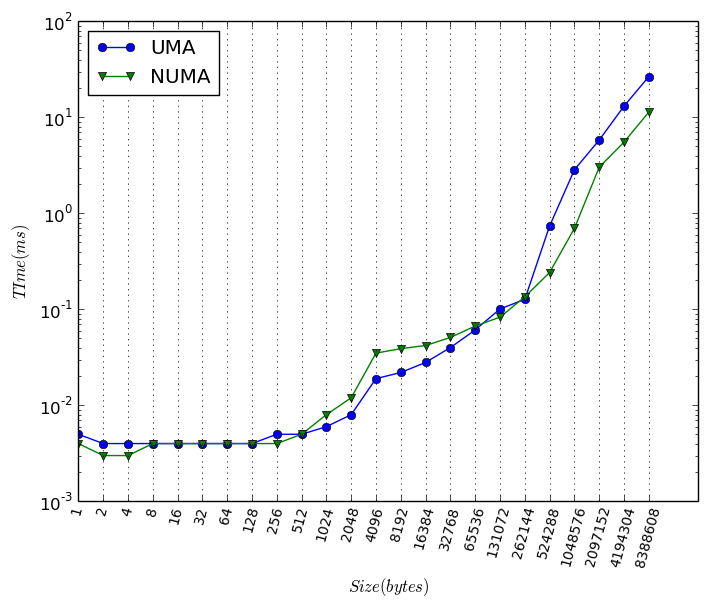
\includegraphics[width=\textwidth]{./images/NUMAvsUMA_alltoall.png}
    \caption{Συγκριτικό διάγραμμα για επικοινωνία σε αρχιτεκτονικές UMA και NUMA για το collective alltoall}
    \label{fig:UMAvsNUMA_alltoall}
\end{figure}
\paragraph{}
 Ακόμη και με μικρό αριθμό διεργασιών, φαίνεται ότι η μοντελοποίηση της επικοινωνίας δεν είναι απλή διαδικασία. Η διάκριση ανάμεσα στους δύο τύπους επικοινωνίας, εσωτερικής του επεξεργαστή και εξωτερικής,  είναι απαραίτητη για να πετύχει κάποιος καλά αποτελέσματα, αφού με βάση την κατανομή των διεργασιών στους πόρους του συστήματος και τα δεδομένα που ανταλλάσσουν, διαφορετικά κομμάτια του συστήματος δέχονται πίεση και άλλα χαρακτηριστικά της αρχιτεκτονικής είναι κυρίαρχα στο χρόνο επικοινωνίας.
\paragraph{}
Έτσι προτείνουμε μία προσέγγιση βασισμένη σε τεχνικές μηχανικής μάθησης, με σκοπό την πρόβλεψη του χρόνου επικοινωνίας MPI εφαρμογών σε αρχιτεκτονική κοινής μνήμης για ασύγχρονη point-to-point αλλά και collective επικοινωνία η οποία διαχωρίζει τις δύο επικοινωνίες.
\paragraph{}
Αποφασίσαμε λοιπόν, να αναλύσουμε την επικοινωνία από τη σκοπιά της MPI εφαρμογής αλλά και τη θέση της στο μηχάνημα. Έτσι ποσοτικοποιούμε τους δύο τύπους επικοινωνίας ξεχωριστά για να μπορούν τα μοντέλα επικοινωνίας που θα αναπτύξουμε να υπολογίζουν την επίδραση της κάθε μίας. Παρόλα αυτά, η μεθοδολογία μας δεν είναι δεσμευτική και θα μπορούσε κάλλιστα να εφαρμοστεί σε δεδομένα εξαγόμενα από το σύστημα εκτέλεσης του MPI. Επιπλέον, η ίδια διαδικασία μπορεί να εφαρμοστεί σε οποιοδήποτε μοντέλο ανταλλαγής μηνυμάτων, χωρίς να είναι απαραίτητη η διάκριση μεταξύ των δύο τύπων επικοινωνίας. Τέλος, πολλά frameworks με σκοπό την ανάλυση μεγάλου όγκου δεδομένων (big data analytics), όπως τα Hama \footnote{http://hama.apache.org} και Pregel \cite{PREGEL}, κάνουν χρήση ενός προγραμματιστικού μοντέλου που ονομάζεται bulk synchonous. Υπολογισμοί και επικοινωνία γίνονται επαναληπτικά σε διακριτές φάσεις με τις διεργασίες να συγχρονίζονται στο τέλος κάθε επανάληψης. Τέτοιου είδους εφαρμογές συνήθως εκτελούνται σε μηχανήματα NUMA μεγάλης κλίμακας, με τη μεθοδολογία μας να είναι ιδανική για πρόβλεψη του χρόνου επικοινωνίας τους. 

\section{Σχετικές Εργασίες}
\paragraph{}
Φυσικά, έχουν προταθεί και άλλες μεθοδολογίες με σκοπό την πρόβλεψη της επίδοσης της επικοινωνίας. Οι περισσότερες ωστόσο, μοντελοποιούν την διαδικασία της επικοινωνίας με χρήση αναλυτικών μοντέλων.
\paragraph{}
Μία πρώτη επιτυχημένη προσπάθεια για πρόβλεψη της point-to-point επικοινωνίας ήταν το μοντέλο του Hockney \cite{HOCKNEY}. Σύμφωνα με το μοντέλο αυτό η καθυστέρηση μπορεί να εκφραστεί σαν:
\begin{align*}
t(s) = t_0 + \frac{s}{b}
\end{align*}
όπου $t$ η καθυστέρηση, $t_0$ η αρχική καθυστέρηση, $s$ το μήκος του μηνύματος και $b$ το μέγιστο εύρος ζώνης (bandwidth) που μπορούμε να πετύχουμε. Ωστόσο, σε σύγχρονες υλοποιήσεις του MPI, το πρωτόκολλο επικοινωνίας αλλάζει ανάλογα με το μήκος του μηνύματος. Κάτι τέτοιο δεν μπορεί να μοντελοποιηθεί από το μοντέλο Hockney καθώς οι παράμετροι του είναι σταθεροί.
\paragraph{}
Μία άλλη προσπάθεια είναι το μοντέλο LogP \cite{LogP}. Πρόκειται για ένα μοντέλο που μπορεί να εφαρμοστεί σε κάθε μηχάνημα και αγνοεί τις λεπτομέρειες της υλοποίησης του πρωτοκόλλου επικοινωνίας. Αποτελείται μόλις από τέσσερις παραμέτρους, την καθυστέρηση (latency - L) ανάμεσα στα modules  για μήνυμα μεγέθους μίας λέξης (συνήθως 8 bytes), το overhead (O), που αφορά το χρόνο που ο επεξεργαστής καταναλώνει για την αποστολή, το κενό (gap - g), που αναπαριστά το ελάχιστο χρονικό διάστημα μεταξύ συνεχόμενων αποστολών μηνυμάτων και τον αριθμό των επεξεργαστών (processors - P). Στις τέσσερις  παραμέτρους που το συνθέτουν οφείλει και το όνομα του. Χρησιμοποιείται κατά κόρο για να δώσει κατευθυντήριες γραμμές  στους σχεδιαστές μηχανημάτων και σαν βάση για γρήγορη ανάπτυξη φορητών παράλληλων αλγορίθμων.

\paragraph{}
Από το 1994, που προτάθηκε το LogP, έχουν αναπτυχθεί πολλές επεκτάσεις του. Οι περισσότερες πρόσθεταν στο μοντέλο νέες παραμέτρους με σκοπό την μοντελοποίηση φαινομένων τα οποία δεν λάμβανε υπόψη.  Το LogGP \cite{LogGP}, προσπαθούσε να συμπεριλάβει τις αλλαγές στο bandwidth για μεγάλα μηνύματα εισάγοντας την παράμετρο G. Επιπλέον της G, το μοντέλο LogGPS  \cite{LogGPS}, έκανε χρήση της παραμέτρου S με σκοπό να συλλάβει αλλαγές στο πρωτόκολλο επικοινωνίας με βάση το μέγεθος του μηνύματος.  

\paragraph{}
Πέραν του LogP και των επεκτάσεων του, που είναι σχεδιασμένα με βάση την τοπολογία της internode επικοινωνίας, μέθοδοι έχουν αναπτυχθεί και για την intranode. Συγκεκριμένα, οι S. Ramos και T. Hoefler \cite{ramos2013modeling}, στην προσπάθεια τους να δώσουν ένα μοντέλο επίδοσης για manycore και multicore αρχιτεκτονικές ανέπτυξαν αναλυτικά μοντέλα για cache-to-cache επικοινωνία. Βασίστηκαν στα πρωτόκολλα που υλοποιούν τη συνοχή της κρυφής μνήμης (cache coherency) τα οποία περιγράφονται με μηχανές πεπερασμένων καταστάσεων. Ανάλογη προσπάθεια, με σκοπό την βελτιστοποίηση της επικοινωνίας έγινε από τον Β. Putigny και άλλους \cite{putigny}. Στόχευαν στη χρήση microbenchmarks με σκοπό την εξαγωγή χαρακτηριστικών της cache καθώς είναι κρίσιμη για την intranode επικοινωνία. Με τα αποτελέσματα μοντελοποίησαν την επικοινωνία πάνω από κοινή μνήμη, επίσης βασιζόμενοι στο πρωτόκολλο συνοχής της κρυφής μνήμης και πρότειναν τεχνικές μέσω των οποίων MPI υλοποιήσεις μπορούν να αυξήσουν την απόδοση της. Τέλος, σε μία πρόσφατη προσπάθεια, αναπτύχθηκε το αναλυτικό μοντέλο \textit{τ-Lop} \cite{tlop}, δίνοντας ένα περίπλοκο μοντέλο επικοινωνίας για collective επικοινωνία χρησιμοποιώντας τους αλγορίθμους που την υλοποιούν, το οποίο παρουσιάζει αξιοσημείωτη ακρίβεια. 

\paragraph{}
Σε γενικές γραμμές, τα αναλυτικά μοντέλα πρέπει να θυσιάσουν την απλότητα τους για να πετύχουν τα αποτελέσματα τους. Καθώς οι αρχιτεκτονικές γίνονται πιο περίπλοκες πρέπει να λαμβάνουν υπόψη τους ακόμα περισσότερα φαινόμενα σε μία ατέλειωτη προσθήκη μεταβλητών. Από την άλλη μεριά, εμπειρικά μοντέλα, που χρησιμοποιούν μετρήσεις από το κάθε μηχάνημα για μοντελοποιήσουν και προβλέψουν την επικοινωνία,  είναι πολύ πιο εύρωστα, παρόλο που απαιτούν εκτέλεση των μετρήσεων σε κάθε μηχάνημα ξεχωριστά. Επιπλέον, αν οι μετρήσεις που περιλαμβάνουν καταφέρνουν να συλλάβουν τα φαινόμενα που διέπουν την επικοινωνία μπορούν να δώσουν πολύ καλά αποτελέσματα με μία σχετικά αυτόματη διαδικασία.
\paragraph{}
Επίσης, σε αναλογία με τα αναλυτικά μοντέλα, μπορούμε να εξετάσουμε και μετρήσεις που αποτυπώνουν τη συμπεριφορά του πρότυπου επικοινωνίας. Αφού πρόκειται για εμπειρικά μοντέλα, θα εντοπίσουν αν κάτι τέτοιο συμβαίνει μέσω των μετρήσεων και θα το μοντελοποιήσουν ανάλογα. 
\paragraph{}
Οι Bhatele και άλλοι \cite{bhatele}, παρουσίασαν πολύ ακριβείς προβλέψεις χρόνου επικοινωνίας, για internode επικοινωνία, κάνοντας χρήση μεθόδων μηχανικής μάθησης. Ωστόσο, η μεθοδολογία τους δεν είναι εφαρμόσιμη για πρόβλεψη πριν την εκτέλεση της εφαρμογής, καθώς χρησιμοποίησαν μετρικές, όπως performance counters, που είναι διαθέσιμες μετά το πέρας της εκτέλεσης της εφαρμογής. Ουσιαστικά σκοπός τους δεν ήταν η πρόβλεψη της επίδοσης της επικοινωνίας, αλλά να προσδιορίσουν τους παράγοντες που επηρεάζουν τη συμφόρηση στα δίκτυα διασύνδεσης.

\section{Περιγραφή Μηχανήματος}
\paragraph{}
Όλα τα πειράματα μας διεξήχθησαν στο μηχάνημα \textit{sandman}. Περιλαμβάνει τέσσερις Intel Xeon E5-4620, τέταρτης γενιάς  συνδεδεμένους  μέσω Intel QuickPath Interconnect. Κάθε ένας από αυτούς αντιστοιχεί σε ένα κόμβο NUMA και διαθέτει 64GiB τοπικής κύριας μνήμης(RAM), με το σύνολο του μηχανήματος να ανέρχεται στα 256GiB. Εντός του κάθε επεξεργαστή υπάρχουν 8 πυρήνες που υποστηρίζουν από δύο νήματα. Κάθε πυρήνας έχει  δύο επίπεδα ιδιωτικής κρυφής μνήμης μεγέθους 32KiB και 256KiB ενώ επιπρόσθετα οι πυρήνες εντός ενός επεξεργαστή μοιράζονται κρυφή μνήμη μεγέθους 16MiB. Μία σχηματική αναπαράσταση του μηχανήματος δίνεται στο Σχημα \ref{fig:sandman}.  
\begin{figure}[ht]
    \centering
    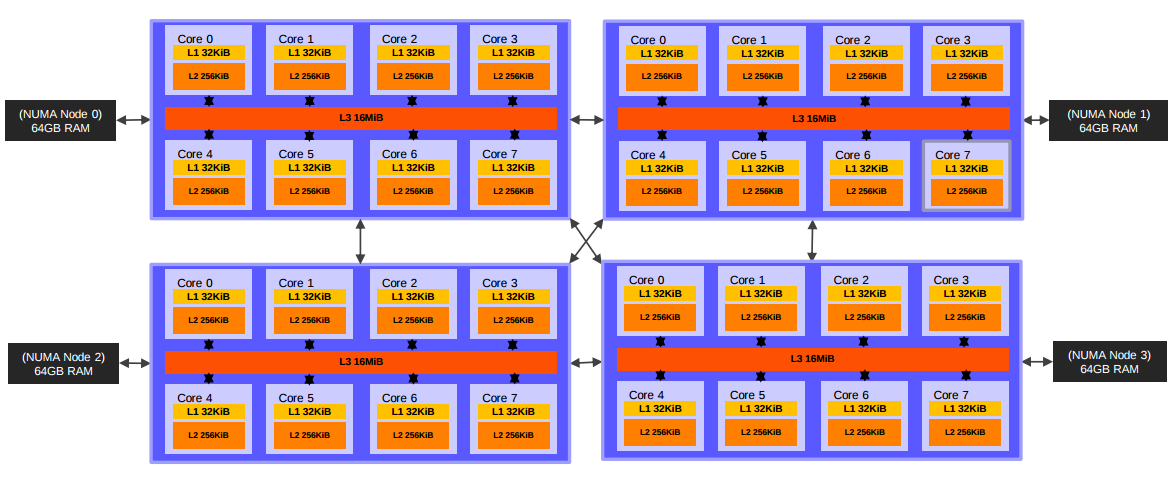
\includegraphics[width=1.1\textwidth]{./images/sandman.png}
    \caption{Αναπαράσταση του μηχανήματος Sandman}
    \label{fig:sandman}
\end{figure}
